\documentclass[12pt]{article}
\usepackage{graphicx}
\usepackage{amsmath}
\usepackage{mathtools}
\usepackage{gensymb}

\newcommand{\mydet}[1]{\ensuremath{\begin{vmatrix}#1\end{vmatrix}}}
\providecommand{\brak}[1]{\ensuremath{\left(#1\right)}}
\providecommand{\norm}[1]{\left\lVert#1\right\rVert}
\newcommand{\solution}{\noindent \textbf{Solution: }}
\newcommand{\myvec}[1]{\ensuremath{\begin{pmatrix}#1\end{pmatrix}}}
\let\vec\mathbf

\begin{document}
\begin{center}
\textbf\large{CONIC SECTIONS}

\end{center}
\section*{Excercise 11.2.4}
	Find the coordinates of the focus, axis of the parabola, the equation of the directrix and the length of the latus rectum of a parabola whose equation is given by $x^2=-16y$.\\

\solution
The given equation of the parabola can be written as
\begin{align}
	\label{eq:parabolaEq1}
	x^2+16y=0
\end{align}
The genereal equation for conic section is
\begin{align}
	\label{eq:parabolaEq2}
	g\brak{\vec{x}}=\vec{x}^\top \vec{V}\vec{x}+2\vec{u}^\top \vec{x}+f=0
\end{align}
Comparaing both equations \eqref{eq:parabolaEq1} and \eqref{eq:parabolaEq2} we get,
\begin{align}
	\label{eq:eqV}
	\vec{V} &= \myvec{1&0\\0&0}\\
	\label{eq:eqU}
	\vec{u} &= \myvec{0\\8}\\
	\label{eq:eqF}
	f &= 0
\end{align}
\begin{enumerate}
\item As   $\vec{V}$ matrix is already diagonalized \eqref{eq:eqV}, the Eigen values $\lambda_1 \text{ and } \lambda_2$ are given as
\begin{align}
	\label{eq:eqEigen1}
	\lambda_1 &= 1\\
	\label{eq:eqEigen2}
	\lambda_2 &= 0
\end{align}
Eigen vector matrix $\vec{P}$ is identical the eigen vector $\vec{P}_2$ by eigen value $\lambda_2$ is 
\begin{align}
	\vec{p}_2 &= \myvec{0\\1}\\
	\vec{n} &= \sqrt{\lambda_1}\vec{p}_2\\
		&= \sqrt{1}\myvec{0\\1}\\
		&= \myvec{0\\1}
\end{align}
So,
\begin{align}
	\label{eq:eqC}
	 \frac{\norm{\vec{u}}^2 - \lambda_1 f}{2\vec{u}^\top \vec{n}}&= c
\end{align}
Substituting  $\vec{u},\vec{n},\lambda_1 \text{ and } f$ values in \eqref{eq:eqC} we get 
\begin{align}
	c = \frac{8^2-1\brak{0}}{2\myvec{0&8}\myvec{0\\1}} = 4
\end{align}
The focus $\vec{F}$ of parabola is 
\begin{align}
	\vec{F} &= \frac{ce^2 \vec{n}-\vec{u}}{\lambda_1}\\
		&= \frac{4\brak{1}^2 \myvec{0\\1}-\myvec{0\\8}}{1}\\
		&= \myvec{0\\-4}
\end{align}
\item Equation of directrix is given as
\begin{align}
	\vec{n}^\top \vec{x} &= c\\
	\myvec{0&1}\vec{x} &= 4\\
	\vec{x}&= 4
\end{align}
\item Equation for tha axis of parabola is 
\begin{align}
	\vec{m}^\top \brak{\vec{x}-\vec{F}} = 0\label{20}
\end{align}
where $\vec{m}$ is the normal vector to the axis and also the slope of the directrix
\begin{align}
	\vec{n} = \myvec{0\\1}\\
	\vec{m} = \myvec{1\\0}
\end{align}
Substituting in \eqref{20}
\begin{align}
	\myvec{1&0}\myvec{\vec{x}-\myvec{0\\-4}}&=0\\
	\myvec{1&0}\vec{x} &= 0\\
	\vec{x}=0
\end{align}
\item Latus rectum of  parabola is 
\begin{align}
	l&=\frac{\eta}{\lambda_1}\\
	 &=\frac{2\vec{u}^\top \vec{p}_2}{\lambda_1}\\
	 &=\frac{2\myvec{0&8}\myvec{0\\1}}{1}\\
	 &=16 \text{ units }
\end{align}
\begin{figure}[!h]
	\begin{center} 
	    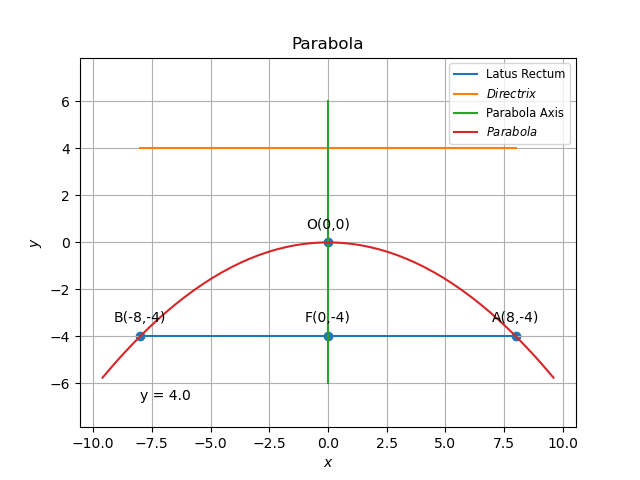
\includegraphics[width=\columnwidth]{figs/parabola}
	\end{center}
\caption{}
\label{fig:Fig1}
\end{figure}
\end{enumerate}
\end{document}
